% Source : http://tex.stackexchange.com/questions/5309/how-can-i-replicate-affine-dynkin-diagrams-in-kacs-textbook

\documentclass{article}
\pagestyle{empty}
\usepackage[paperheight=40cm,scale=.97]{geometry}
\usepackage{amssymb}
\usepackage{mathtools}
\usepackage{tikz}
\usetikzlibrary{chains}

\tikzset{node distance=2em, ch/.style={circle,draw,on chain,inner sep=2pt},chj/.style={ch,join},every path/.style={shorten >=4pt,shorten <=4pt},line width=1pt,baseline=-1ex}

\newcommand{\alabel}[1]{%
  \(\alpha_{\mathrlap{#1}}\)
}

\newcommand{\mlabel}[1]{%
  \(#1\)
}

\let\dlabel=\alabel
\let\ulabel=\mlabel

\newcommand{\dnode}[2][chj]{%
\node[#1,label={below:\dlabel{#2}}] {};
}

\newcommand{\dnodea}[3][chj]{%
\dnode[#1,label={above:\ulabel{#2}}]{#3}
}

\newcommand{\dnodeanj}[2]{%
\dnodea[ch]{#1}{#2}
}

\newcommand{\dnodenj}[1]{%
\dnode[ch]{#1}
}

\newcommand{\dnodebr}[1]{%
\node[chj,label={below right:\dlabel{#1}}] {};
}

\newcommand{\dnoder}[2][chj]{%
\node[#1,label={right:\dlabel{#2}}] {};
}

\newcommand{\dydots}{%
\node[chj,draw=none,inner sep=1pt] {\dots};
}

\newcommand{\QRightarrow}{%
\begingroup
\tikzset{every path/.style={}}%
\tikz \draw (0,3pt) -- ++(1em,0) (0,1pt) -- ++(1em+1pt,0) (0,-1pt) -- ++(1em+1pt,0) (0,-3pt) -- ++(1em,0) (1em-1pt,5pt) to[out=-75,in=135] (1em+2pt,0) to[out=-135,in=75] (1em-1pt,-5pt);
\endgroup
}

\newcommand{\QLeftarrow}{%
\begingroup
\tikz
\draw[shorten >=0pt,shorten <=0pt] (0,3pt) -- ++(-1em,0) (0,1pt) -- ++(-1em-1pt,0) (0,-1pt) -- ++(-1em-1pt,0) (0,-3pt) -- ++(-1em,0) (-1em+1pt,5pt) to[out=-105,in=45] (-1em-2pt,0) to[out=-45,in=105] (-1em+1pt,-5pt);
\endgroup
}

\begin{document}
\begin{align*}
A_l &&& 
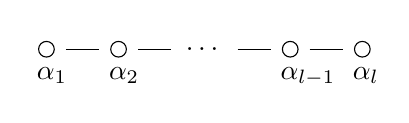
\begin{tikzpicture}[start chain]
\dnode{1}
\dnode{2}
\dydots
\dnode{l-1}
\dnode{l}
\end{tikzpicture}
&&
(l+1) \\
%
B_l &&&
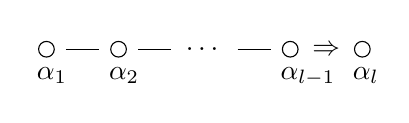
\begin{tikzpicture}[start chain]
\dnode{1}
\dnode{2}
\dydots
\dnode{l-1}
\dnodenj{l}
\path (chain-4) -- node[anchor=mid] {\(\Rightarrow\)} (chain-5);
\end{tikzpicture}
&&
(2) \\
%
C_l &&&
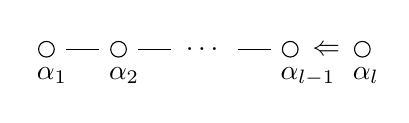
\begin{tikzpicture}[start chain]
\dnode{1}
\dnode{2}
\dydots
\dnode{l-1}
\dnodenj{l}
\path (chain-4) -- node[anchor=mid] {\(\Leftarrow\)} (chain-5);
\end{tikzpicture}
&&
(2) \\
%
D_l &&&
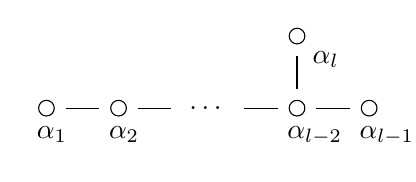
\begin{tikzpicture}
\begin{scope}[start chain]
\dnode{1}
\dnode{2}
\node[chj,draw=none] {\dots};
\dnode{l-2}
\dnode{l-1}
\end{scope}
\begin{scope}[start chain=br going above]
\chainin(chain-4);
\dnodebr{l}
\end{scope}
\end{tikzpicture}
&&
(4) \\
%
E_6 &&&
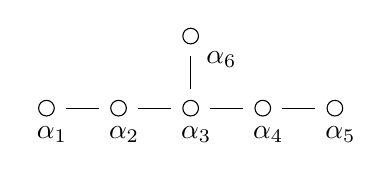
\begin{tikzpicture}
\begin{scope}[start chain]
\foreach \dyni in {1,...,5} {
\dnode{\dyni}
}
\end{scope}
\begin{scope}[start chain=br going above]
\chainin (chain-3);
\dnodebr{6}
\end{scope}
\end{tikzpicture}
&&
(3) \\
%
E_7 &&&
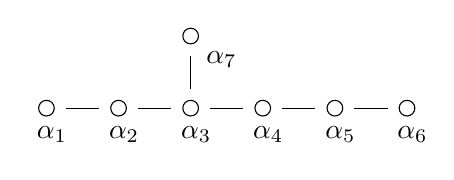
\begin{tikzpicture}
\begin{scope}[start chain]
\foreach \dyni in {1,...,6} {
\dnode{\dyni}
}
\end{scope}
\begin{scope}[start chain=br going above]
\chainin (chain-3);
\dnodebr{7}
\end{scope}
\end{tikzpicture}
&&
(2) \\
%
E_8 &&&
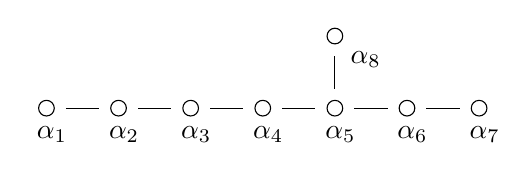
\begin{tikzpicture}
\begin{scope}[start chain]
\foreach \dyni in {1,...,7} {
\dnode{\dyni}
}
\end{scope}
\begin{scope}[start chain=br going above]
\chainin (chain-5);
\dnodebr{8}
\end{scope}
\end{tikzpicture}
&&
(1) \\
%
F_4 &&&
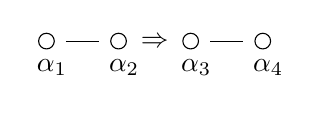
\begin{tikzpicture}[start chain]
\dnode{1}
\dnode{2}
\dnodenj{3}
\dnode{4}
\path (chain-2) -- node[anchor=mid] {\(\Rightarrow\)} (chain-3);
\end{tikzpicture}
&&
(1) \\
%
G_2 &&&
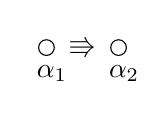
\begin{tikzpicture}[start chain]
\dnodenj{1}
\dnodenj{2}
\path (chain-1) -- node {\(\Rrightarrow\)} (chain-2);
\end{tikzpicture}
\end{align*}

\let\dlabel=\mlabel

\begin{align*}
&A_1^{(1)} &&
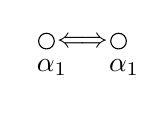
\begin{tikzpicture}[start chain]
\dnodenj{1}
\dnodenj{1}
\path (chain-1) -- node[anchor=mid] {\(\Longleftrightarrow\)} (chain-2);
\end{tikzpicture}
\\
%
&A_l^{(1)} (l \ge 2) &&
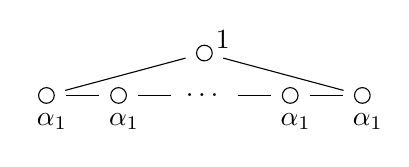
\begin{tikzpicture}[start chain,node distance=1ex and 2em]
\dnode{1}
\dnode{1}
\dydots
\dnode{1}
\dnode{1}
\begin{scope}[start chain=br going above]
\chainin(chain-3);
\node[ch,join=with chain-1,join=with chain-5,label={[inner sep=1pt]10:\(1\)}] {};
\end{scope}
\end{tikzpicture}
\\
%
&B_l^{(1)} (l \ge 3) &&
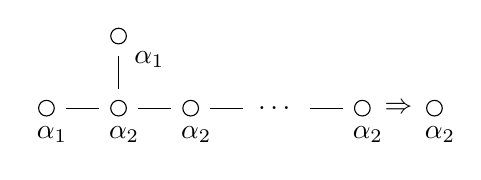
\begin{tikzpicture}
\begin{scope}[start chain]
\dnode{1}
\dnode{2}
\dnode{2}
\dydots
\dnode{2}
\dnodenj{2}
\end{scope}
\begin{scope}[start chain=br going above]
\chainin(chain-2);
\dnodebr{1}
\end{scope}
\path (chain-5) -- node{\(\Rightarrow\)} (chain-6);
\end{tikzpicture}
\\
%
&C_l^{(1)} (l \ge 2) &&
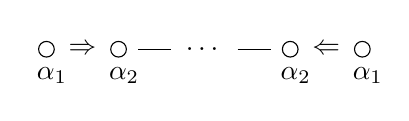
\begin{tikzpicture}[start chain]
\dnodenj{1}
\dnodenj{2}
\dydots
\dnode{2}
\dnodenj{1}
\path (chain-1) -- node{\(\Rightarrow\)} (chain-2);
\path (chain-4) -- node{\(\Leftarrow\)} (chain-5);
\end{tikzpicture}
\\
%
&D_l^{(1)} (l \ge 4) &&
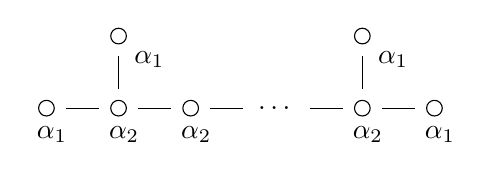
\begin{tikzpicture}
\begin{scope}[start chain]
\dnode{1}
\dnode{2}
\dnode{2}
\dydots
\dnode{2}
\dnode{1}
\end{scope}
\begin{scope}[start chain=br going above]
\chainin(chain-2);
\dnodebr{1};
\end{scope}
\begin{scope}[start chain=br2 going above]
\chainin(chain-5);
\dnodebr{1};
\end{scope}
\end{tikzpicture}
\\
%
&G_2^{(1)} &&
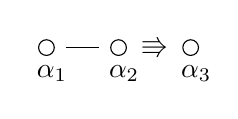
\begin{tikzpicture}[start chain]
\dnode{1}
\dnode{2}
\dnodenj{3}
\path (chain-2) -- node{\(\Rrightarrow\)} (chain-3);
\end{tikzpicture}
\\
%
&F_4^{(1)} &&
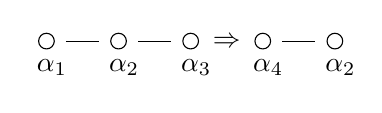
\begin{tikzpicture}[start chain]
\dnode{1}
\dnode{2}
\dnode{3}
\dnodenj{4}
\dnode{2}
\path (chain-3) -- node[anchor=mid]{\(\Rightarrow\)} (chain-4);
\end{tikzpicture}
\\
%
&E_6^{(1)} &&
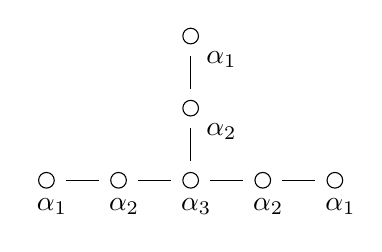
\begin{tikzpicture}
\begin{scope}[start chain]
\foreach \dyi in {1,2,3,2,1} {
\dnode{\dyi}
}
\end{scope}
\begin{scope}[start chain=br going above]
\chainin(chain-3);
\dnodebr{2}
\dnodebr{1}
\end{scope}
\end{tikzpicture}
\\
%
&E_7^{(1)} &&
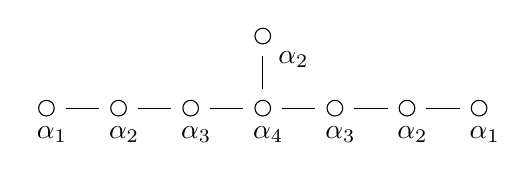
\begin{tikzpicture}
\begin{scope}[start chain]
\foreach \dyi in {1,2,3,4,3,2,1} {
\dnode{\dyi}
}
\end{scope}
\begin{scope}[start chain=br going above]
\chainin(chain-4);
\dnodebr{2}
\end{scope}
\end{tikzpicture}
\\
%
&E_8^{(1)} &&
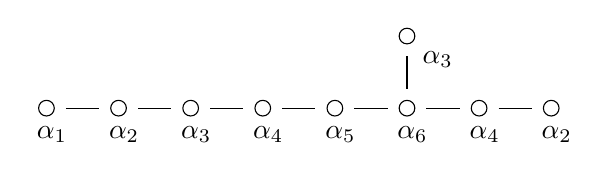
\begin{tikzpicture}
\begin{scope}[start chain]
\foreach \dyi in {1,2,3,4,5,6,4,2} {
\dnode{\dyi}
}
\end{scope}
\begin{scope}[start chain=br going above]
\chainin(chain-6);
\dnodebr{3}
\end{scope}
\end{tikzpicture}
\end{align*}

\let\dlabel=\alabel

\begin{align*}
&A_2^{(2)} &&
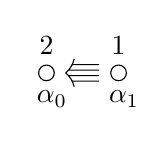
\begin{tikzpicture}[start chain]
\dnodeanj{2}{0}
\dnodeanj{1}{1}
\path (chain-1) -- node {\QLeftarrow} (chain-2);
\end{tikzpicture}
\\
%
&A_{2l}^{(2)} (l \ge 2) &&
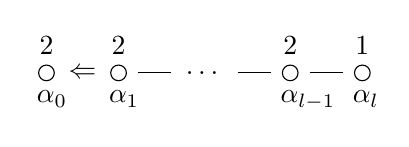
\begin{tikzpicture}[start chain]
\dnodeanj{2}{0}
\dnodeanj{2}{1}
\dydots
\dnodea{2}{l-1}
\dnodea{1}{l}
\path (chain-1) -- node[anchor=mid] {\(\Leftarrow\)} (chain-2);
\end{tikzpicture}
\\
%
&A_{2l-1}^{(2)} (l \ge 3) &&
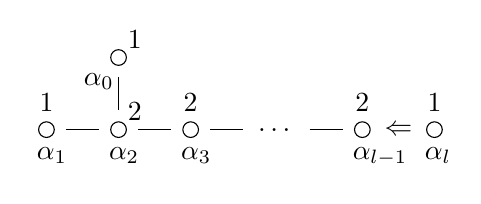
\begin{tikzpicture}
\begin{scope}[start chain]
\dnodea{1}{1}
\node[chj,label={below:\dlabel{2}},label={[inner sep=1pt]above right:\mlabel{2}}] {};
\dnodea{2}{3}
\dydots
\dnodea{2}{l-1}
\dnodeanj{1}{l}
\path (chain-5) -- node[anchor=mid] {\(\Leftarrow\)} (chain-6);
\end{scope}
\begin{scope}[start chain=br going above]
\chainin(chain-2);
\node[chj,label={below left:\dlabel{0}},label={[inner sep=1pt]above right:\mlabel{1}}] {};
\end{scope}
\end{tikzpicture}
\\
%
&D_{l+1}^{(2)} (l \ge 2) &&
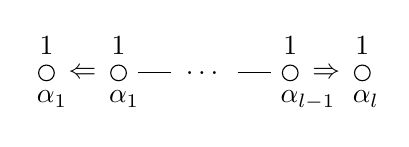
\begin{tikzpicture}[start chain]
\dnodea{1}{1}
\dnodeanj{1}{1}
\dydots
\dnodea{1}{l-1}
\dnodeanj{1}{l}
\path (chain-1) -- node[anchor=mid] {\(\Leftarrow\)} (chain-2);
\path (chain-4) -- node[anchor=mid] {\(\Rightarrow\)} (chain-5);
\end{tikzpicture}
\\
%
&E_6^{(2)} &&
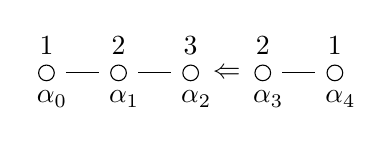
\begin{tikzpicture}[start chain]
\dnodea{1}{0}
\dnodea{2}{1}
\dnodea{3}{2}
\dnodeanj{2}{3}
\dnodea{1}{4}
\path (chain-3) -- node[anchor=mid] {\(\Leftarrow\)} (chain-4);
\end{tikzpicture}
\end{align*}

\begin{align*}
&D_4^{(3)} &&
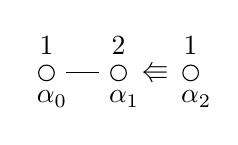
\begin{tikzpicture}[start chain]
\dnodea{1}{0}
\dnodea{2}{1}
\dnodeanj{1}{2}
\path (chain-2) -- node {\(\Lleftarrow\)} (chain-3);
\end{tikzpicture}
\end{align*}

\end{document}
